\chapter{Commandes de bases}

Dans cette partie, nous allons voir les commandes de bases qui permettent de se débroullier dans un terminal.


À la différence de Windows, le terminal est un outils très utilisé sous linux. Il permet de :
\begin{itemize}
	\item se déplacer dans l'arborescence des fichiers
	\item créer/supprimer des dossiers
	\item créer/éditer/supprimer des fichiers
\end{itemize}

Évidemment il existe des outils graphiques pour effectuer ces différentes tâches mais parfois il peut être plus rapide de faire ces actions diretement dans le terminal.

\section{pwd (print working directory)}
Cette commande permet de savoir où l'on se situe dans l'arborescence.

\begin{center}
	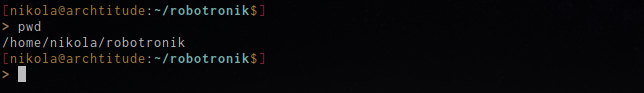
\includegraphics[width=0.6\textwidth]{Images/pwd.png}
	\captionof{figure}{Sortie de la commande pwd}
\end{center}

\section{ls}
Cette commande permet de lister les éléments présents dans un dossier.

\begin{center}
	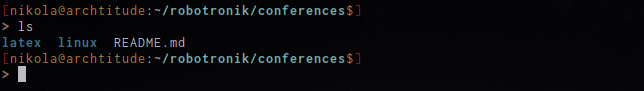
\includegraphics[width=0.6\textwidth]{Images/ls.png}
	\captionof{figure}{Sortie de la commande ls}
\end{center}

Il est possible d'ajouter des flags (drapeaux) à cette commande. Les flags sont des options que l'on peut affecter à une commande. La plupart du temps, la liste des flags affectable à une commande peuvent être trouver dans le manuel de cette commande.

Par exemple, si l'on ajoute le flag -a :

\begin{center}
	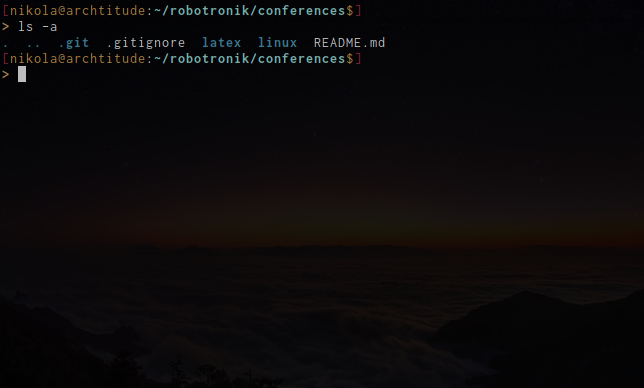
\includegraphics[width=0.6\textwidth]{Images/ls-a.png}
	\captionof{figure}{Sortie de la commande ls -a}
\end{center}

De nouveaux fichiers sont apparus. Le nom de ces fichiers est précédé d'un point. Cela signifie que ce sont des fichiers cachés. Si l'on demande pas de les afficher explicitement il ne seront pas visibles.

Plusieurs flags peuvent être utilisés en même temps. Par exemple, si l'on entre la commande :
\begin{lstlisting}[language=bash]
	ls -al
\end{lstlisting}

\begin{center}
	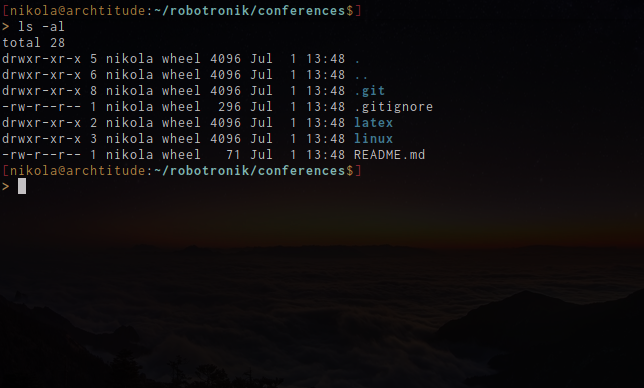
\includegraphics[width=0.6\textwidth]{Images/ls-al.png}
	\captionof{figure}{Sortie de la commande ls -al}
\end{center}

Ici, les fichiers cachés sont toujours affiché car nous avons mis le flag a mais l'affichage est changé. Cela est dû au flag -l qui permet d'obtenir plus d'inofrmation sur les fichiers commes leur taille, leurs autirisations, leur propriétaire et leur date de dernière modification.

\section{cd (change directory)}
Cette commande permet - comme son nom l'indique - de changer de dossier.

\begin{center}
	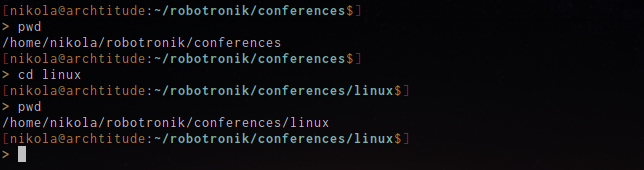
\includegraphics[width=0.6\textwidth]{Images/cd.png}
	\captionof{figure}{Sortie de la commande cd}
\end{center}

\section{mkdir (make directory) / rmdir (remove directory)}
Ces deux commandes permettent de créer et supprimer des dossiers.

\begin{center}
	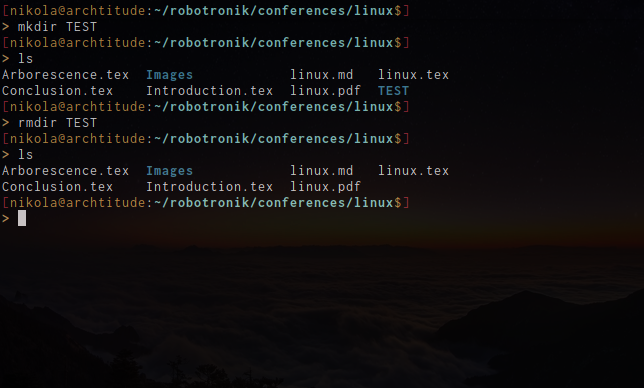
\includegraphics[width=0.6\textwidth]{Images/dir.png}
	\captionof{figure}{Création puis suppression d'un dossier}
\end{center}

Attention pour utiliser rmdir, il faut que le dossier que l'on veut supprimer soit vide. Sinon il faut utiliser la commande rm (cf \ref{sec:touch-rm})

\section{touch/rm}\label{sec:touch-rm}
Ces deux commandes permettent de créer et supprimer des fichiers. 

La commande touch ne permet de créer que des fichiers et non des dossiers. Pour créer un fichier il faut entrer cette commande :
\begin{lstlisting}[language=bash]
	touch nom_de_mon_fichier.extention_de_mon_fichier
\end{lstlisting}

Par exemple, disons que l'on veut créer un fichier pour ecrire un programme en C :

\begin{center}
	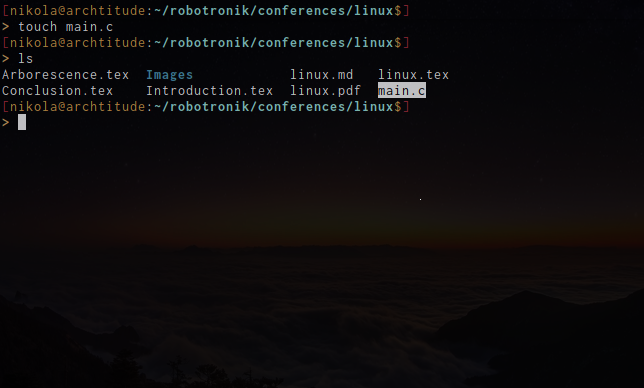
\includegraphics[width=0.6\textwidth]{Images/touch.png}
	\captionof{figure}{Création du fichier main.c}
\end{center}

La commande rm permet de supprimer un élément. Elle pernet aussi de supprimer des dossiers non vide en lui affectant les bons flags.

\begin{center}
	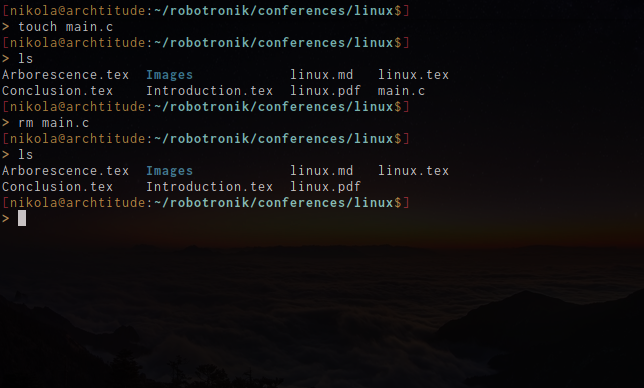
\includegraphics[width=0.6\textwidth]{Images/rm.png}
	\captionof{figure}{Suppression du fichier crée précédement}
\end{center}

